%%
%% Copyright 2007, 2008, 2009 Elsevier Ltd
%%
%% This file is part of the 'Elsarticle Bundle'.
%% ---------------------------------------------
%%
%% It may be distributed under the conditions of the LaTeX Project Public
%% License, either version 1.2 of this license or (at your option) any
%% later version.  The latest version of this license is in
%%    http://www.latex-project.org/lppl.txt
%% and version 1.2 or later is part of all distributions of LaTeX
%% version 1999/12/01 or later.
%%
%% The list of all files belonging to the 'Elsarticle Bundle' is
%% given in the file `manifest.txt'.
%%

%% Template article for Elsevier's document class `elsarticle'
%% with numbered style bibliographic references
%% SP 2008/03/01
%%
%%
%%
%% $Id: elsarticle-template-num.tex 4 2009-10-24 08:22:58Z rishi $
%%
%%

\documentclass[preprint,12pt]{elsarticle}

%% Use the option review to obtain double line spacing
%% \documentclass[preprint,review,12pt]{elsarticle}

%% Use the options 1p,twocolumn; 3p; 3p,twocolumn; 5p; or 5p,twocolumn
%% for a journal layout:
%% \documentclass[final,1p,times]{elsarticle}
%% \documentclass[final,1p,times,twocolumn]{elsarticle}
%% \documentclass[final,3p,times]{elsarticle}
%% \documentclass[final,3p,times,twocolumn]{elsarticle}
%% \documentclass[final,5p,times]{elsarticle}
%% \documentclass[final,5p,times,twocolumn]{elsarticle}

%% if you use PostScript figures in your article
%% use the graphics package for simple commands
%% \usepackage{graphics}
%% or use the graphicx package for more complicated commands
%% \usepackage{graphicx}
%% or use the epsfig package if you prefer to use the old commands
%% \usepackage{epsfig}

%% The amssymb package provides various useful mathematical symbols
\usepackage{amssymb}
\usepackage[colorlinks]{hyperref}
\hypersetup{citecolor=DeepPink4}
\hypersetup{linkcolor=DarkRed}
\hypersetup{urlcolor=DarkBlue}
\usepackage{hyperref}
\usepackage{caption}
\usepackage{cleveref}
\usepackage{subcaption}


%% The amsthm package provides extended theorem environments
%% \usepackage{amsthm}

%% The lineno packages adds line numbers. Start line numbering with
%% \begin{linenumbers}, end it with \end{linenumbers}. Or switch it on
%% for the whole article with \linenumbers after \end{frontmatter}.
%% \usepackage{lineno}

%% natbib.sty is loaded by default. However, natbib options can be
%% provided with \biboptions{...} command. Following options are
%% valid:

%%   round  -  round parentheses are used (default)
%%   square -  square brackets are used   [option]
%%   curly  -  curly braces are used      {option}
%%   angle  -  angle brackets are used    <option>
%%   semicolon  -  multiple citations separated by semi-colon
%%   colon  - same as semicolon, an earlier confusion
%%   comma  -  separated by comma
%%   numbers-  selects numerical citations
%%   super  -  numerical citations as superscripts
%%   sort   -  sorts multiple citations according to order in ref. list
%%   sort&compress   -  like sort, but also compresses numerical citations
%%   compress - compresses without sorting
%%
%% \biboptions{comma,round}

% \biboptions{}


\journal{Intelligent Data Analysis (extended)}

\begin{document}

\begin{frontmatter}

%% Title, authors and addresses

%% use the tnoteref command within \title for footnotes;
%% use the tnotetext command for the associated footnote;
%% use the fnref command within \author or \address for footnotes;
%% use the fntext command for the associated footnote;
%% use the corref command within \author for corresponding author footnotes;
%% use the cortext command for the associated footnote;
%% use the ead command for the email address,
%% and the form \ead[url] for the home page:
%%
%% \title{Title\tnoteref{label1}}
%% \tnotetext[label1]{}
%% \author{Name\corref{cor1}\fnref{label2}}
%% \ead{email address}
%% \ead[url]{home page}
%% \fntext[label2]{}
%% \cortext[cor1]{}
%% \address{Address\fnref{label3}}
%% \fntext[label3]{}

\title{Partitioning the Parts of a Pizza}

%% use optional labels to link authors explicitly to addresses:
%% \author[label1,label2]{<author name>}
%% \address[label1]{<address>}
%% \address[label2]{<address>}

\author{Amar Lakshya (Student ID: 2096845)}

\address{School of Computer Science, University of Birmingham}

\begin{abstract}
Pizza is one of the most popular fast food in the world. In this report, experiments were conducted over a sample pizza dataset
to develop a better understanding of the various attributes of pizza and their relationships. A number of data-analysis techniques
like Principal Component Analysis and co-ordinate projections were employed to understand the characteristics of  10 anonymized 
brand names in the dataset and 7 different attributes of each pizza.
\end{abstract}

\begin{keyword}
%% keywords here, in the form: keyword \sep keyword
Food \sep Pizza \sep PCA
%% MSC codes here, in the form: \MSC code \sep code
%% or \MSC[2008] code \sep code (2000 is the default)

\end{keyword}

\end{frontmatter}

%%
%% Start line numbering here if you want
%%
% \linenumbers

%% main text
\section{Acknowledgement}
\label{s:acknowledge}
I would like to thank  Prof. Martin Russell for this educational and challenging assignment, and  Dhilip Subramanian for his pizza dataset.

\section{Introduction}
\label{s:introduction}
The story of making food in a Pizza like fashion goes back to the Neolithic Age \cite{pizzaOrigins1991}. There have been several
notable instances of Pizza consumption in almost all kinds of cultures ranging from the Persian to the Greeks \cite{Persian2014} \cite{Greek2000}
Although, it's perfectly clear that pizza consumption has only increased in the recent times and toppings choices have 
been extensively discussed, a lot of attributes of the food still remains hidden. 
\par
\section{Research Questions}
\label{s:ResearchQuestions}
Through this project, we aim to explore those attributes and their relationships that might influence qualitative aspects of a Pizza.
Consequently, we aim to answer the following questions:

\begin{itemize}
\item Which attribute/attributes most explains the difference between the brands of Pizzas?
\item How does attributes affect each other and affect the brands of Pizzas?
\item What are the different amount of attributes present in different brands of Pizzas?
\end{itemize}

\section{Methods}
\label{s:Methods}
The results were obtained by using the following python tools (libraries):  \textit{numpy, pandas, matplotlib, sklearn}. \cite{softwares}
\par
The entire source code of the project containing the generated images and the analysis can be found at: \href{https://github.com/amar-laksh/UNI/tree/master/assignments/IDA/assignment}{Github}.
\section{Dataset}
\label{s:Dataset}
The sample dataset has been retrieved from the \href{https://data.world/sdhilip/pizza-datasets}{Data World website}. 
The dataset is in the \textbf{\textit{csv}} file format and is \textbf{``\textit{,}'' }separated It is comprised of the following columns:
\begin{enumerate}
\item \textbf{brand} -- Pizza brand (class label)
\item \textbf{id} -- Sample analysed
\item \textbf{mois} -- Amount of water per 100 grams in the sample
\item \textbf{prot} -- Amount of protein per 100 grams in the sample
\item \textbf{fat} -- Amount of fat per 100 grams in the sample
\item \textbf{ash} -- Amount of ash per 100 grams in the sample
\item \textbf{sodium} -- Amount of sodium per 100 grams in the sample
\item \textbf{carb} -- Amount of carbohydrates per 100 grams in the sample
\item \textbf{cal} -- Amount of calories per 100 grams in the sample
\end{enumerate}
\par
The following things are to be noted about the dataset:
\begin{itemize}
\item The \textbf{\textit{id}} attribute has been removed from the data-set since it doesn't  especially contribute to the analysis of the data.
\item The \textbf{\textit{brand}} attribute is the class label that already comes with the dataset and thus can be used initially.
\end{itemize}
\section{Preprocessing}
\label{ss:Preprocessing}
In order to investigate the data any further it was necessary to first check whether the entire dataset had standardised values. To do this, the
scale of the measurements of the data had to be checked. This was done by creating a box plot which can be seen in Figure~\ref{fig:raw_boxplot}.
\par
As is seen from the figure, all the attributes contribute different units to the data and therefore it was necessary to standardize the data.
\par
Standardisation for this dataset was done using the \textit{preprocessing} class from the \textit{sklearn} library \cite{scaling2020}  and applying the \textit{fitTransform} 
function. After applying the standardisation, a new box plot was produced and can be seen in Figure~\ref{fig:scaled_boxplot.png}. 

\section{Labelling}
\label{ss:Labelling}
Since the original dataset came labelled with the class field \textit{brand}, there was no need for a labelling scheme and the values in the \textit{set} of \textit{brand} namely:
\textit{A', 'B', 'C', 'D', 'E', 'F', 'G', 'H', 'I', 'J'} were used.

\section{Principal Component Analysis}
\label{ss:PrincipalComponentAnalysis}
The standardised data was then put through the \textit{pca} function of the \textit{sklearn} library \cite{pca2020} to generate the eigenvectors, eigenvalues, and the coefficients
of the eigenvalues. To find the most useful eigenvectors from the PCA step, a scree plot of the percentage of variance was plotted and can be seen in Figure~\ref{fig:scree_plot.png}.
\par
As can be seen from the scree plot, the first two principal components namely: \textit{PC1, PC2} contribute nearly \textbf{59\% }and \textbf{32\% }of variances respectively.
Therefore, only these two principal components were chosen for further analysis.
\par
A 2D projection was then generated to cover all the classes through the two chosen principal components and can be seen in Figure~\ref{fig:pca_projection.png}.
This can be considered a good result as various clusters of different classes can be uniquely identified. It might be improved further by adding another principal component
but since the percentage of variance was too low, such a decision was not considered wise.
\par
A biplot was also generated to show both the coefficients of the eigenvalues for each attribute and the principal component score for each data point and can be 
seen in Figure~\ref{fig:bi_plot.png}. Furthermore, Table~\ref{table:eigenvectors} and Table~\ref{table:eigenvalues} show the corresponding eigenvectors and eigenvalues.
\par
The direction and the length of vectors produced indicates the contribution to the principal components from each attribute. For example it can be observed from Fig ~\ref{fig:bi_plot.png} that attributes such as \textit{mois, cal, prot, fat, ash, sodium} being on the the right side of the y-axis most contributed to \textit{PC1}, while 
\textit{carb, fat} being above the x-axis most contributed to \textit{PC2}.
\section{Coordinate Projections}
\label{ss:CoordinateProjections}
 As vectors close to each are bound to have strong correlations, A 2D projection of the closest
pair namely, \textit{fat} and \textit{sodium} was generated and can be seen in Fig ~\ref{fig:fat_sodium.png}. It did look promising and hence 2D projections for all
combination of the attributes were generated to be studied. ( They can be found at \href{https://github.com/amar-laksh/UNI/tree/master/assignments/IDA/assignment/gen_images/attributes}{Github}). Consequently, \textit{mois} was found to be the most important attribute in all the 2D projections as can be seen from Fig ~\ref{fig:mois} since it clearly separates classes across all attributes.
\par
It is also worth stating that as clear from the biplot, the \textit{mois }vector makes a relatively small angle with \textit{prot }and \textit{ash }vectors and they seem to be positively
correlated. This can also be verified by looking at the 2D projections for \textit{prot} and \textit{ash} (especially with \textit{mois}) in which both act as good attributes to cluster the different classes neatly.
\section{Histogram Analysis}
\label{ss:HistogramAnalysis}
Histograms for each attribute frequency for all the classes were generated and analysed (They can be found at \href{https://github.com/amar-laksh/UNI/tree/master/assignments/IDA/assignment/gen_images/histograms}{Github}). Consequently, a few observations were made:
\begin{itemize}
\item The histogram for \textit{mois} attribute shown in Fig~\ref{fig:brands_all.png} , clearly demonstrates that this attribute captures all the class values effectively
\item The histogram in Fig~\ref{fig:brands_all.png} for \textit{fat, sodium }and \textit{cal} clearly shows segmented positive values for the \textit{brand A}. These three attributes can also be seen contributing the most to the PC1 principal component as shown from the Fig~\ref{fig:bi_plot.png} as welll as Table ~\ref{table:eigenvectors}.
\item The histograms in Fig~\ref{fig:brands_all.png} also shows that \textit{brand} classes \textit{G, H, I} have the most negative values in the \textit{fat, sodium, cal} attributes. \item The historgrams also show that the brand classes \textit{G, H, I} have positive values  for only the \textit{carb }attribute. Furthermore, From Fig ~\ref{fig:bi_plot.png},  and  Table~\ref{table:eigenvectors} , we can see that \textit{carb }  contributes the most to PC2.
\end{itemize}

\section{Conclusion}
\label{s:Conclusion}
Standardisation of data was necessary and all calculations were based on the standardised dataset.
The following were the observations noted at the conclusion:
\begin{itemize}
\item Adding a 3rd principal component can increase the accuracy of predictions.
\item Projections of \textit{mois} seems to be the best method to predict different brands of pizzas in the dataset.
\item There seems to be close relationships between \textit{fat, sodium, cal } attributes as derived from PCA.
\item Brand \textit{A} seems to be easy to predict using PC1 and usually contains high amounts of \textit{fat, } \textit{sodium }and \textit{cal}.
\item Brand \textit{G, H, I} seem to be predicted by using PC2 and are usually low in \textit{fat, sodium }and \textit{cal} values.
\item \textit{mois, ash, prot} seem to be a good set of predictors for classes.
\item Further clustering techniques can definitely be applied to the dataset to procure more knowledge based on the 2D projections produced.
\end{itemize}
%% The Appendices part is started with the command \appendix;
%% appendix sections are then done as normal sections
%% \appendix

%% \section{}
%% \label{}

%% References
%%
%% Following citation commands can be used in the body text:
%% Usage of \cite is as follows:
%%   \cite{key}         ==>>  [#]
%%   \cite[chap. 2]{key} ==>> [#, chap. 2]
%%

%% References with bibTeX database:

\bibliographystyle{elsarticle-num}
%\bibliography{<your-bib-database>}

%% Authors are advised to submit their bibtex database files. They are
%% requested to list a bibtex style file in the manuscript if they do
%% not want to use elsarticle-num.bst.

%% References without bibTeX database:

\begin{thebibliography}{00}
%% \bibitem must have the following form:
%%   \bibitem{key}...
%%
\bibitem{pizzaOrigins1991} Perry, C. {\em A Stone-Age Snack : History: Pizza topped with tomatoes, pepperoni and cheese is only 100 years old}. Los Angeles Times,1991
\bibitem{Persian2014} Barrett, L  {\em Pizza, A Slice of American History}, 2014,13.
\bibitem{Greek2000} Buonassisi, R. {\em Pizza: From its Italian Origins to the Modern Table. Firefly.} , 2000, 78.
\bibitem{softwares} \href{https://numpy.org/}{NymPy}, \href{https://pandas.pydata.org/}{Pandas},\href{https://matplotlib.org/}{Matplotlib}, \href{https://scikit-learn.org/stable/index.html}{Scikit-learn}
\bibitem{scaling2020} \href{https://scikit-learn.org/stable/auto_examples/preprocessing/plot_scaling_importance.html}{Importance of Scaling}
\bibitem{pca2020} \href{https://scikit-learn.org/stable/modules/generated/sklearn.decomposition.PCA.html}{Sci-kit learn PCA function docs}
\end{thebibliography}

\begin{figure}[b]
	\centering
    \centerline{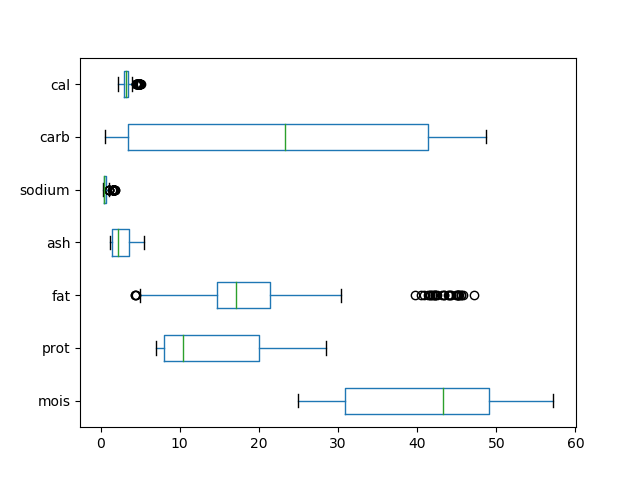
\includegraphics[scale=0.6]{figs/raw_boxplot.png}}
    \caption{A box plot showing the raw ranges of the dataset}\label{fig:raw_boxplot}
\end{figure}

\begin{figure}[hb]
	\centering
    \centerline{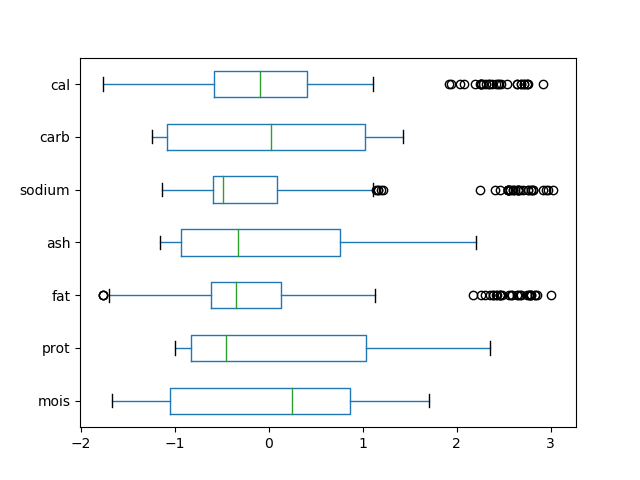
\includegraphics[scale=0.6]{figs/scaled_boxplot.png}}
    \caption{A box plot showing the standardised values of the dataset}\label{fig:scaled_boxplot.png}
\end{figure}

\begin{figure}[hb]
	\centering
    \centerline{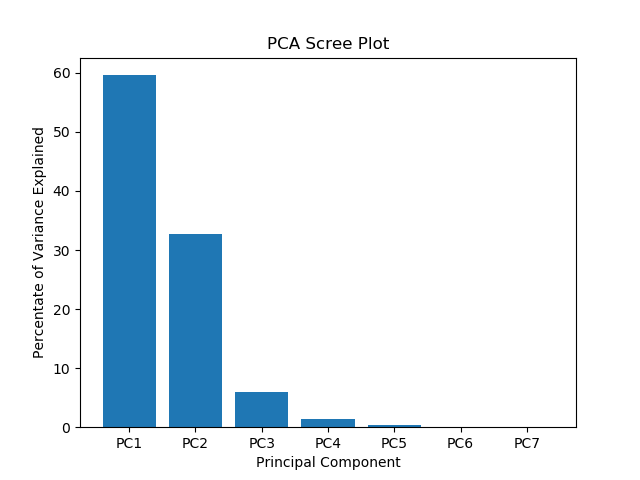
\includegraphics[scale=0.6]{figs/scree_plot.png}}
    \caption{A scree plot over the various principal components}\label{fig:scree_plot.png}
\end{figure}

\begin{figure}[hb]
	\centering
    \centerline{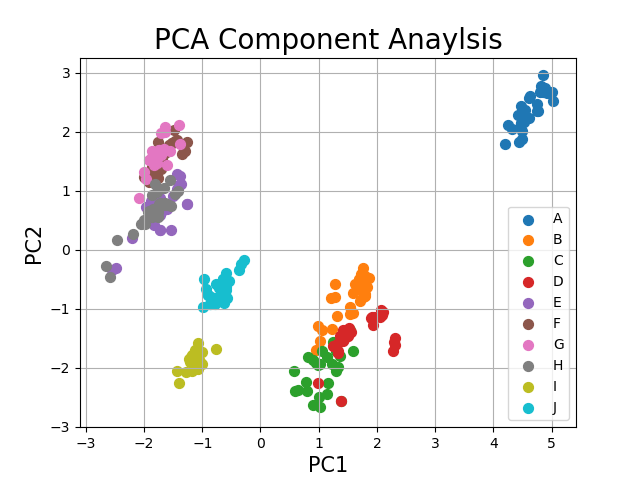
\includegraphics[scale=0.6]{figs/pca_projection.png}}
    \caption{A 2D Projection over the  two Principal Components}\label{fig:pca_projection.png}
\end{figure}

\begin{figure}[hb]
	\centering
    \centerline{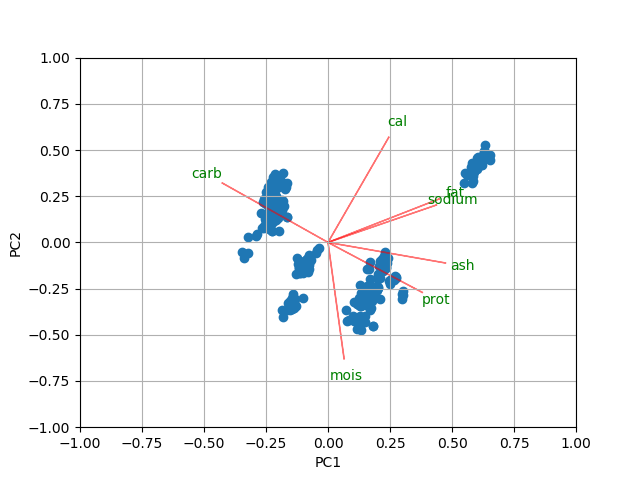
\includegraphics[scale=0.6]{figs/bi_plot.png}}
    \caption{A biplot presenting the coefficients for each attribute}\label{fig:bi_plot.png}
\end{figure}


\begin{figure}[hb]
	\centering
    \centerline{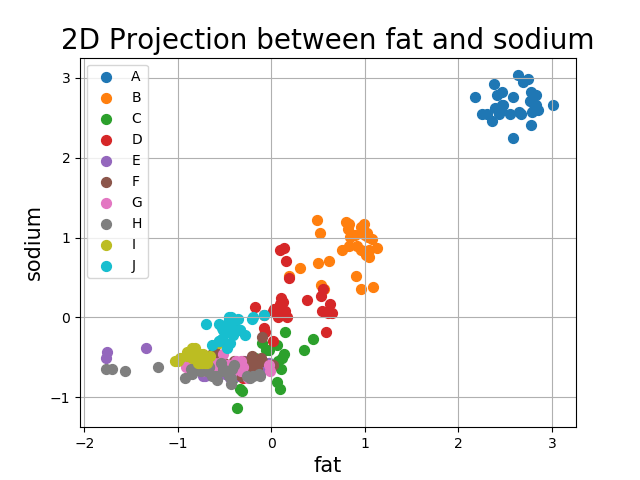
\includegraphics[scale=0.6]{figs/fat_sodium.png}}
    \caption{A 2D Projection over Fat and Sodium}\label{fig:fat_sodium.png}
\end{figure}


\begin{figure}[hb]
	\centering
	\subfloat {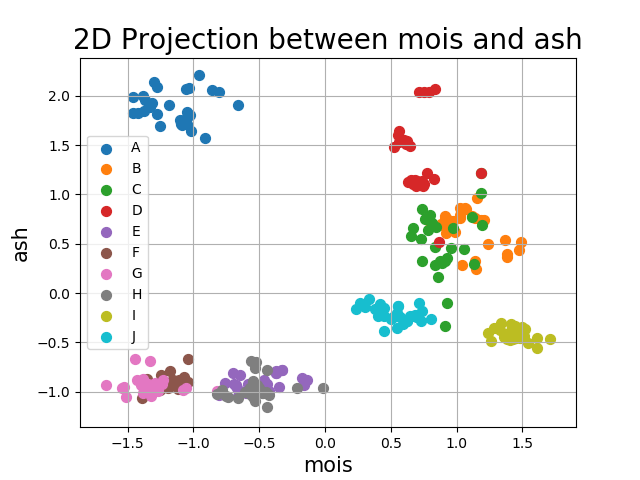
\includegraphics[width=4cm]{figs/mois_ash.png}}
	\subfloat{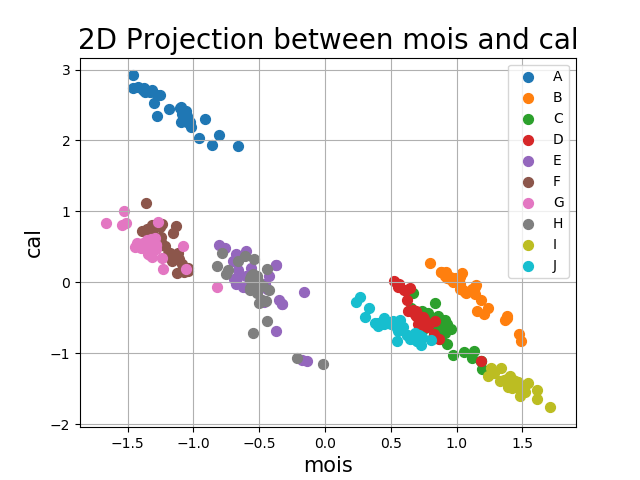
\includegraphics[width=4cm]{figs/mois_cal.png}}
	\qquad	
	\subfloat{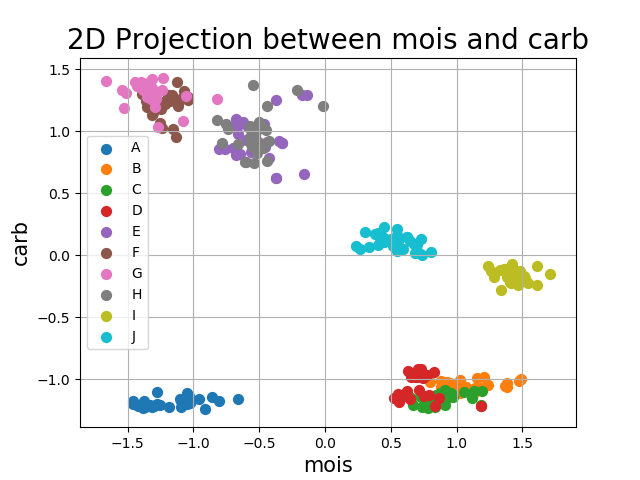
\includegraphics[width=4cm]{figs/mois_carb.png}}
	\subfloat{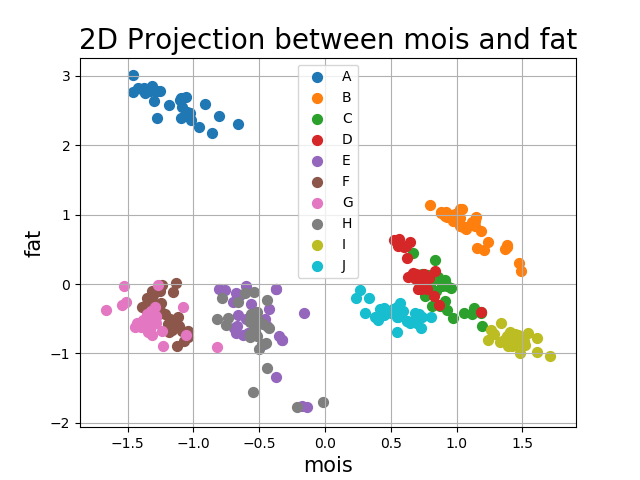
\includegraphics[width=4cm]{figs/mois_fat.png}}
    \qquad
	\subfloat{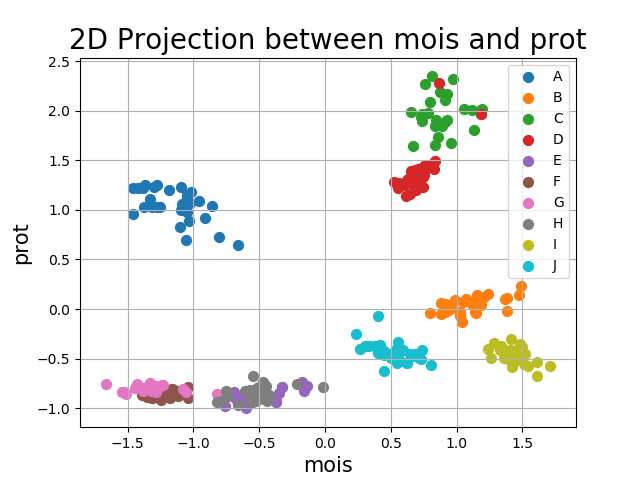
\includegraphics[width=4cm]{figs/mois_prot.png}}
	\subfloat{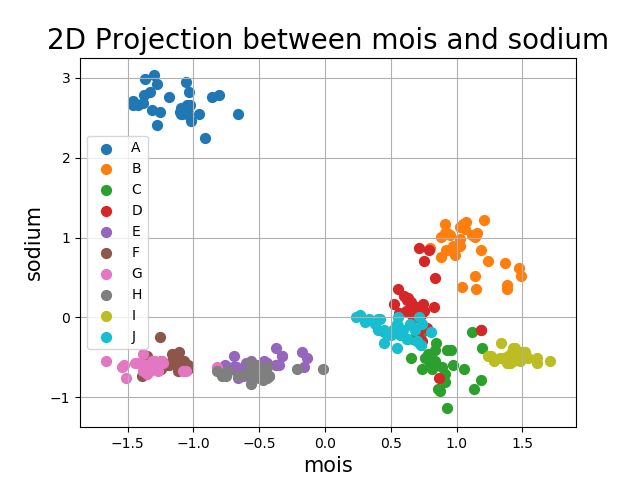
\includegraphics[width=4cm]{figs/mois_sodium.png}}
    \caption{2D Projections of \textit{mois} with other attributes}
    \label{fig:mois}
\end{figure}

\begin{figure}[hb]
	\centering
	\subfloat{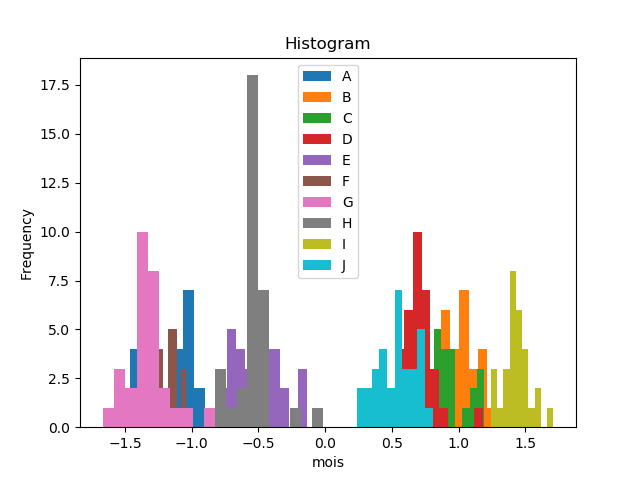
\includegraphics[width=8cm]{figs/brands_mois.png}}
	\qquad
	\subfloat {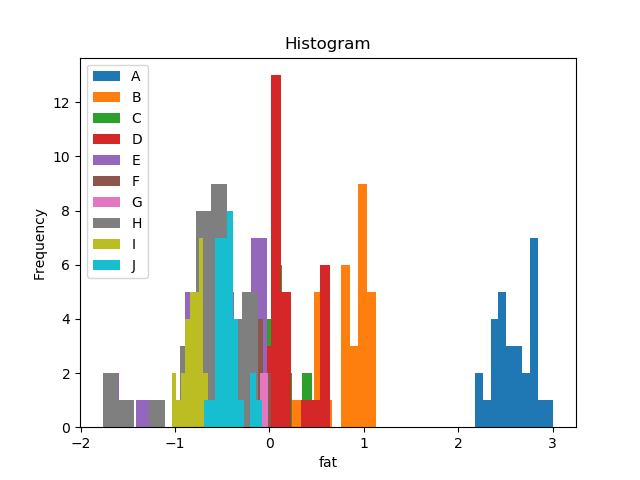
\includegraphics[width=5cm]{figs/brands_fat.png}}
	\subfloat{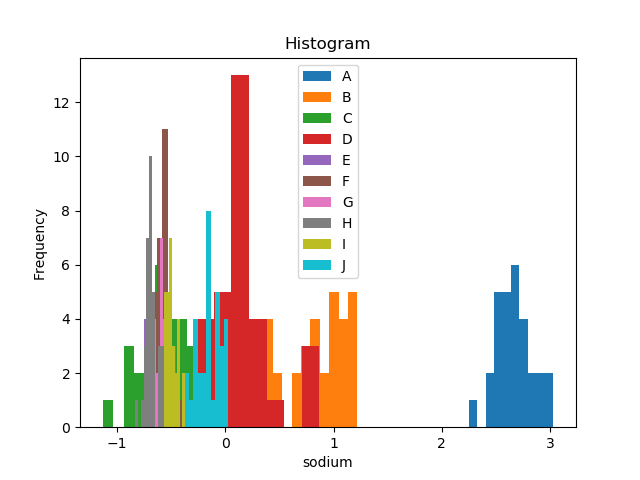
\includegraphics[width=5cm]{figs/brands_sodium.png}}
	\subfloat{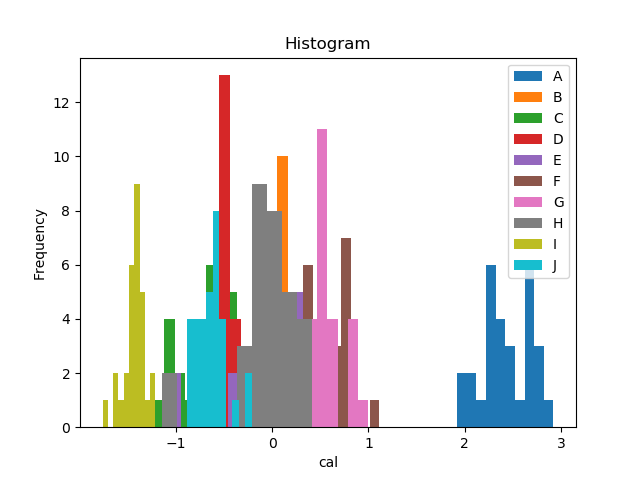
\includegraphics[width=5cm]{figs/brands_cal.png}}
	\qquad	
	\subfloat{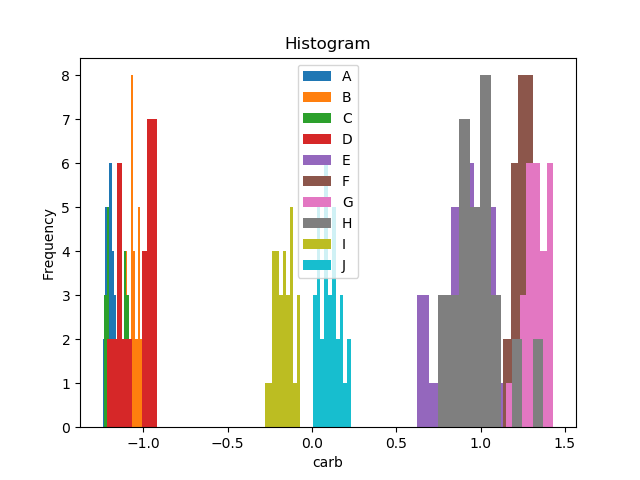
\includegraphics[width=5cm]{figs/brands_carb.png}}
	\subfloat{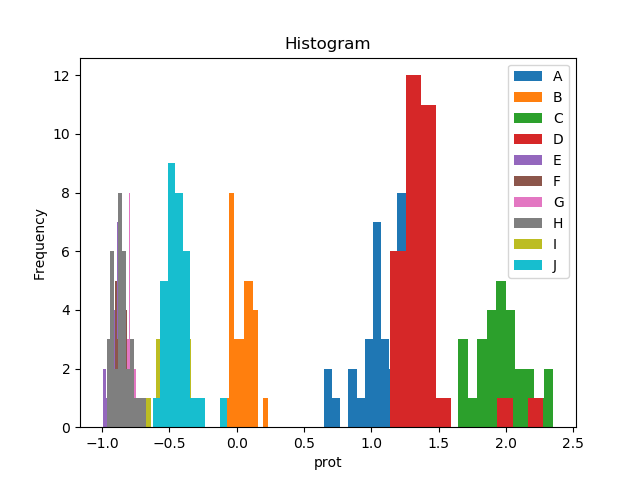
\includegraphics[width=5cm]{figs/brands_prot.png}}
	\subfloat{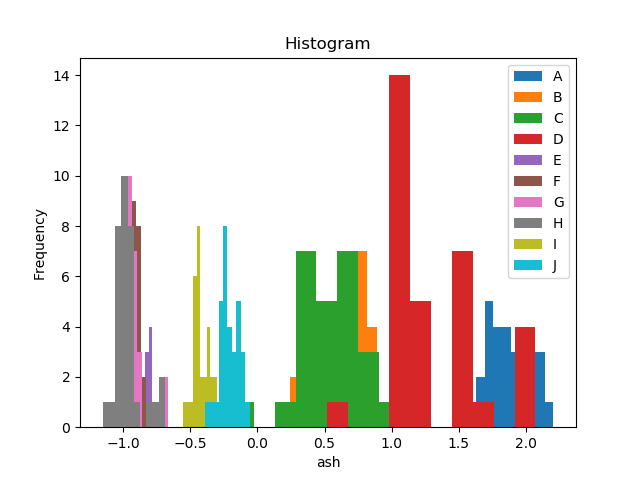
\includegraphics[width=5cm]{figs/brands_ash.png}}
	
    \caption{Histograms of \textit{mois, fat, sodium, cal, carb, prot, ash}}
    \label{fig:brands_all.png}
\end{figure}


\begin{table}[h!]
\centering
\begin{tabular}{ |c| |c| |c| |c| |c| |c| |c| |c|}
\hline
 PCs & mois & prot & fat & ash & sodium & carb & cal \\ [0.2ex] 
 \hline
 PC1 & 0.064709 & 0.378761 & 0.446666 & 0.471890  & 0.435703 & -0.424914 & 0.244487 \\
 PC2 & -0.628276 & -0.269707 & 0.234379 & -0.110990  & 0.201662  & 0.320312  & 0.567458 \\
 PC3 & -0.421669 & 0.746027 & -0.199309 & 0.056273 & -0.455169 & 0.052237 & 0.113316 \\
 PC4 & -0.220722 & -0.010593 & -0.507042 & 0.552399 & 0.446277 & 0.334339 & -0.279263 \\
 PC5 & -0.006470 & -0.387983 & 0.173368 & 0.670886 & -0.602614 & 0.007437 & 0.078003 \\
 PC6 & 0.446450 & -0.000172 & -0.525403 & 0.058861 & 0.003131 & -0.000509 & 0.721914 \\
 PC7 & 0.418569 & 0.276765 & 0.377672 & 0.056021 & -0.000524 & 0.776068 & 0.012060 \\ [1ex]
  \hline\hline
\end{tabular}
\caption{Table showing PCA eigenvectors for each attribute}\label{table:eigenvectors}
\end{table}

\begin{table}[h!]
\centering
\begin{tabular}{ |c| |c| }
\hline
 PCs & brand\\ [0.2ex] 
 \hline
PC1 & 4.185734 \\
PC2 & 2.298118 \\
PC3 & 0.415949 \\
PC4 & 0.095493 \\
PC5 & 0.027770 \\ 
PC6 & 0.000339 \\
PC7 & 0.000010 \\
  \hline\hline
\end{tabular}
\caption{Table showing PCA eigenvalues over the class}\label{table:eigenvalues}
\end{table}

\end{document}

%%
%% End of file `elsarticle-template-num.tex'.
